
%
%
%     File Name :
%
%       Purpose :
%
% Creation Date :
%
% Last Modified : Tue 05 Mar 2013 05:21:43 PM ART
%
%    Created By :  Ezequiel Castillo
%
%

\documentclass[a4paper,12pt]{article}

\usepackage[utf8x]{inputenc}
\usepackage[spanish,activeacute,es-noshorthands]{babel} % Caracteres conacentos. Modificado E. Castillo.
\usepackage{amsmath,amssymb,amsfonts,amsthm,latexsym,cancel,chemarrow} %Soporte para símbolos y font matemáticos
\usepackage{verbatim}
\usepackage{color}
%\usepackage{wrapfig}
%\usepackage{graphicx}
\usepackage{hyperref}
%\usepackage{threeparttable} %Footnotes en las tablas
%\usepackage{booktabs}          
%\usepackage{multirow} 
%\usepackage{rotating}
%\usepackage{listings} % Ambiente para incluir Codigo Fuente 
\usepackage{a4wide}
%\usepackage{sidecap} %Side Caption
%\usepackage[scriptsize,bf]{caption} %Caption negrita y chiquita
%\usepackage{tikz}
%\usetikzlibrary{calc,3d}
%\usepackage{gnuplot-lua-tikz}
%\usepackage{grffile} %Para leer archivo .algo.pdf
%\usepackage{array}
%\usepackage[version=3]{mhchem}
%\usepackage{setspace}
%\onehalfspacing
\usepackage{parskip}
\usepackage{mdframed}
\usepackage{framed}
\usepackage{enumerate}

\usepackage{xstring}

\setlength{\parindent}{15pt}
\setlength{\parskip}{1ex plus 0.5ex minus 0.2ex}


%******MY COMMANDS*******
\DeclareMathOperator{\tr}{tr}
\newcommand{\bi}[1]{\textbf{\emph{#1}}}
\newcommand{\xvec}[0]{\textbf{x}}
\newcommand{\demo}{\noindent\textbf{Demostración: }}
\newcommand{\obse}{\noindent\textsc{Observación: }}

%******MY ENVIRONMENTS*******
\newenvironment{concept}[1][]{%
  \begin{framed}
  \IfStrEq{#1}{i}{\itshape}{}%
  }{%
  \end{framed}}%

\newmdtheoremenv[linewidth=2,skipbelow=2ex,skipabove=2ex]{theorem}{Teorema}
\usepackage{blindtext}

%*****MY COLORS*****
\definecolor{mygreen}{RGB}{0,117,0}
\definecolor{myviolet}{RGB}{200,193,249}
\definecolor{mylightyellow}{RGB}{249,248,193}


\graphicspath{{img/}} 
\DeclareGraphicsExtensions{.pdf,.png,.jpg}


%\lstdefinelanguage{Git}{
  %basicstyle=\small\ttfamily,
  %breaklines=true,
  %frame=single,
  %morestring=[b]',
  %moredelim=[is][\color{red}\ttfamily]{|}{|},
  %moredelim=[is][\color{gray}\ttfamily]{||}{||},
  %framerule=0pt,
  %rulesep=4pt,
  %framextopmargin=4pt,
  %framexbottommargin=4pt,
  %aboveskip=2ex,
  %belowskip=1ex,
  %numbers=none,  % where to put the line-numbers; possible values are (none, left, right)
  %%numbersep=0pt,
  %%numberstyle=\tiny\color{gray},
  %%stepnumber=2,
  %tabsize=4,
  %classoffset=0,
  %keywords={git},
  %keywordstyle=\color{blue}\bfseries,
  %classoffset=1,
  %morekeywords={remote, add, clone, rename, rm, fetch, pull, 
                %push, commit}, keywordstyle=\color{mygreen}\bfseries,
  %classoffset=0,
  %sensitive=false,
  %%stringstyle=\ttfamily
%}
%\lstdefinestyle{input}
  %{ 
  %backgroundcolor=\color{myviolet},
  %}
%\lstdefinestyle{output}
  %{
  %backgroundcolor=\color{mylightyellow},
  %identifierstyle=\color{gray} 
  %}

%\lstset{language=Git}


\begin{document}


\title{Resúmen de álgebra lineal} 
\date{\today}
\author{Castillo, M. Ezequiel}

\maketitle


\section{Intro}

En una simulación de Dinámica Molecular (DM) uno elige un potencial
interatómico apropiado para describir las fuerzas entre los átomos y luego
integra las ecuaciones clásicas de movimiento con condiciones de contorno
apropiadas. Una característica particular de la DM es que sigue la verdadera
evolución del sistema. Sin embargo, la limitación del tiempo de simulación
accesible representa un obstáculo sustancial en cuanto a la predicción de
ciertas propiedades. Para tener en cuenta las vibraciones atómicas es
necesario utilizar un paso de tiempo cercano al femtosegundo, de modo que
simular un microsegundo es bastante difícil hoy en día. Incluso utilizando
cálculos paralelizados se alcanzan normalmente tiempos del orden de
nanosegundos.


Una posible alternativa para sobreponerse a este inconveniente lo constituye
la ``dinámica  aceleradaLa'' en donde la trayectoria del sistema, atrapada en su estado
actual, es simulada para encontrar una ruta apropiada para escapar más
rápidamente que si lo hiciera con una DM directa. No se necesita información a
priori acerca de cómo es la ruta de escape en el procedimiento; la trajectoria
simplemente sigue su propio camino fuera de su estado.

%------------------------------------------
%------------------------------------------

\section{Background}

\subsection{Sistemas de eventos infrecuentes}

La evolución dinámica de un sistema consiste en excursiones vibracionales
dentro de un valle (o pozo) de potencial, interrumpidas por transiciones ocasionales
entre los valles; estos eventos son infrecuentes en el sentido de que se
necesita en promedio un tiempo muy largo de períodos vibracionales. En algún
punto del tiempo, cuando se localiza la suficiente energía, la trayectoria pasa
a través de una superficie divisoria. La dimensión de un sistema es
$3N$-dimensional. Una trayectoria en este espacio de coordenadas
$3N$-dimensional necesita pasar indefectiblemente por una cordillera de
dimensiones $(3N-1)$-dimensional para llegar a otro valle. Sin embargo a veces
pueden ocurrir sucesivos cruzamientos en tan sólo un período vebracional o
dos. Estos son denominados eventos dinámicos correlacionados. En la mayoría de
los métodos de Dinámica Acelerada (DA) asumimos que estos eventos correlacionados
no ocurren (esta es una de las suposiciones más importantes de la Teoría del
Estado de Transición, TST). Por lo tanto se define un tiempo de correlación
($\tau_{corr}$) del sistema como la duración de memoria del sistema. Una
trayectoria que haya residido un tiempo mayor a $\tau_{corr}$ quiere decir que
el sistema se ha olvidado de cómo llegó ahí (es decir, que la probabilidad de
salir de un valle es independiente de cómo llegó allí).

La búsqueda que ocurre dentro de un pozo de potencial puede implicar un número
grande de excursiones vibracionales. La llave de la DA es reconocer que para
encontrar la secuencia correcta de transiciones de estado a estado, no es
necesario recrear la dinámica vibracional perfectamente, siempre y cuando la
probabilidad de encontrar cada una de las rutas de escape se mantenga.

\begin{SCfigure}
	\centering
	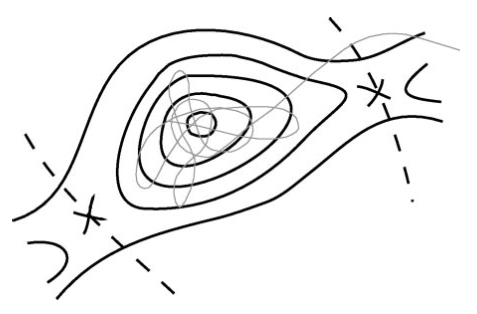
\includegraphics[width=8cm]{basin.png}
	\caption{En esencia, el sistema ``accidentalmente'' escapa del estado y
	una nueva sesión de búsqueda vibracional empieza, sin memoria de cómo
	llegó a ese estado.}
	\label{fig:basin}
\end{SCfigure}

%------------------------------------------
\end{document}
